\begin{frame}
	\myheading{Module 9.5 : Batch Normalization}
\end{frame}

%%%%%%%%%%%%%%%%%%%%%%%%%%%%%%%%%%%%%%%%%%%%%%%%%%%%%%%%%%%%%%%%%%%%%%%%%%%%%%%%%%%%%%%%%
			
\begin{frame}
	We will now see a method called batch normalization which allows us to be less careful about initialization
\end{frame}

%Batch Normalization
\begin{frame}
	
	\begin{columns}
		
		\column{0.35\textwidth}
		\begin{overlayarea}{\textwidth}{\textheight}						
			\only<2-7>{
				\tikzstyle{input_neuron}=[circle,draw=black!50,fill=black!10,thick,minimum size=6mm]
\tikzstyle{hidden_neuron}=[circle,draw=blue!50,fill=blue!10,thick,minimum size=6mm]
\tikzstyle{output_neuron}=[circle,draw=green!50,fill=green!20,thick,minimum size=6mm]
\tikzstyle{hidden_neuron1}=[circle,draw=red!50,fill=red!10,thick,minimum size=6mm]
\tikzstyle{input}=[circle,draw=black!50,fill=black!20,thick,minimum size=6mm]

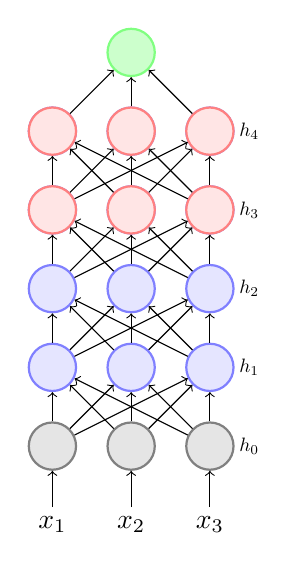
\begin{tikzpicture}
	
	\node [input_neuron] (in1) at (6,-2) {};
	\node [input_neuron] (in2) at (7,-2) {};
	\node [input_neuron] (in3) at (8,-2) {};
	\node [hidden_neuron] (h01) at (6,-1) {};
	\node [hidden_neuron] (h02) at (7,-1) {};
	\node [hidden_neuron] (h03) at (8,-1) {};
	\node [hidden_neuron] (h11) at (6,0) {};
	\node [hidden_neuron] (h12) at (7,0) {};
	\node [hidden_neuron] (h13) at (8,0) {};
	\node [hidden_neuron] (h21) at (6,1) {};
	\node [hidden_neuron] (h22) at (7,1) {};
	\node [hidden_neuron] (h23) at (8,1) {};
	\node [hidden_neuron] (h31) at (6,2) {};
	\node [hidden_neuron] (h32) at (7,2) {};
	\node [hidden_neuron] (h33) at (8,2) {};
	\node (input1) at (6,-3)  {$x_{1}$};
	\node (input2) at (7,-3)  {$x_{2}$};
	\node (input3) at (8,-3)  {$x_{3}$};
	\node [output_neuron] (o1) at (7,3) {};
	\draw [->] (input1) -- (in1);
	\draw [->] (input2) -- (in2);
	\draw [->] (input3) -- (in3);
	
	\draw [->] (in1) -- (h01);
	\draw [->] (in1) -- (h02);
	\draw [->] (in1) -- (h03);
	\draw [->] (in2) -- (h01);
	\draw [->] (in2) -- (h02);
	\draw [->] (in2) -- (h03);
	\draw [->] (in3) -- (h01);
	\draw [->] (in3) -- (h02);
	\draw [->] (in3) -- (h03);
	
	\draw [->] (h01) -- (h11);
	\draw [->] (h01) -- (h12);
	\draw [->] (h01) -- (h13);
	\draw [->] (h02) -- (h11);
	\draw [->] (h02) -- (h12);
	\draw [->] (h02) -- (h13);
	\draw [->] (h03) -- (h11);
	\draw [->] (h03) -- (h12);
	\draw [->] (h03) -- (h13);
	
	\draw [->] (h11) -- (h21);
	\draw [->] (h11) -- (h22);
	\draw [->] (h11) -- (h23);
	\draw [->] (h12) -- (h21);
	\draw [->] (h12) -- (h22);
	\draw [->] (h12) -- (h23);
	\draw [->] (h13) -- (h21);
	\draw [->] (h13) -- (h22);
	\draw [->] (h13) -- (h23);
	
	\draw [->] (h21) -- (h31);
	\draw [->] (h21) -- (h32);
	\draw [->] (h21) -- (h33);
	\draw [->] (h22) -- (h31);
	\draw [->] (h22) -- (h32);
	\draw [->] (h22) -- (h33);
	\draw [->] (h23) -- (h31);
	\draw [->] (h23) -- (h32);
	\draw [->] (h23) -- (h33);
	\draw [->] (h31) -- (o1);
	\draw [->] (h32) -- (o1);
	\draw [->] (h33) -- (o1);
	
	
	\node (formula)[scale=.7] at (8.5,-2) {$h_{0}$};
	
	\node (formula)[scale=.7] at (8.5,-1) {$h_{1}$};
	\node (formula)[scale=.7] at (8.5, 0) {$h_{2}$};
	\node (formula)[scale=.7] at (8.5,1) {$h_{3}$};
	\node (formula)[scale=.7] at (8.5,2) {$h_{4}$};
	
	\only<3->{
		\node [hidden_neuron1] (h21) at (6,1) {};
		\node [hidden_neuron1] (h22) at (7,1) {};
		\node [hidden_neuron1] (h23) at (8,1) {};
		\node [hidden_neuron1] (h31) at (6,2) {};
		\node [hidden_neuron1] (h32) at (7,2) {};
		\node [hidden_neuron1] (h33) at (8,2) {};
	}
	
\end{tikzpicture}
			}
			
		\end{overlayarea}
		
		
		\column{0.65\textwidth}
		
		\begin{overlayarea}{\textwidth}{\textheight}
			\only<1-7>{
				\begin{itemize}
					\justifying
					\only<1->{\item To understand the intuition behind Batch Normalization let us consider a deep network}
					\only<3->{\item Let us focus on the learning process for the weights between these two layers}
					\only<4->{\item Typically we use mini-batch algorithms}
					\only<5->{\item What would happen if there is a constant change in the distribution of $h_3$}
					\only<6->{\item In other words what would happen if across mini-batches the distribution of $h_3$ keeps changing}
					\only<7->{\item Would the learning process be easy or hard?}
				\end{itemize}
			}
			
		\end{overlayarea}
	\end{columns}
\end{frame}

%%%%%%%%%%%%%%%%%%%%%%%%%%%%%%%%%%%%%%%%%%%%%%%%%%%%%%%%%%%%%%%%%%%%%%%%%%%%%%%%%%%%%%%%%			

\begin{frame}
	\begin{columns}
		\column{0.35\textwidth}
		\begin{overlayarea}{\textwidth}{\textheight}
			\only<1-8>{
				\only<1>{
					\begin{figure}
						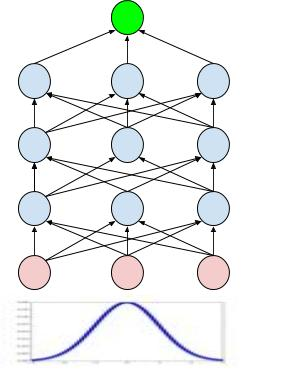
\includegraphics[scale=0.3]{images/BN_no.jpg}
					\end{figure}
				}
				\only<2>{
					\begin{figure}
						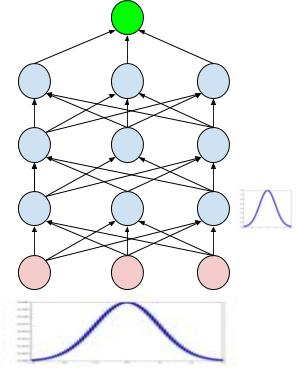
\includegraphics[scale=0.3]{images/BN_1.jpg}
					\end{figure}
				}
				\only<3>{
					\begin{figure}
						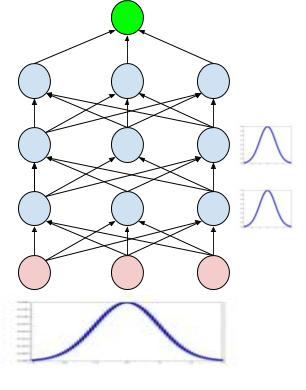
\includegraphics[scale=0.3]{images/BN_2.jpg}
					\end{figure}
				}
				\only<4>{
					\begin{figure}
						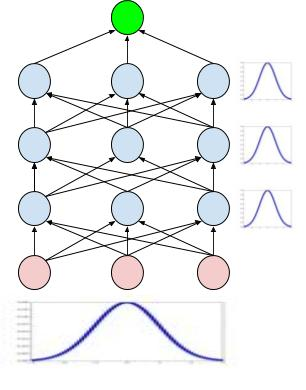
\includegraphics[scale=0.3]{images/BN_3.jpg}
					\end{figure}
				}
				\only<5->{
					\begin{figure}
						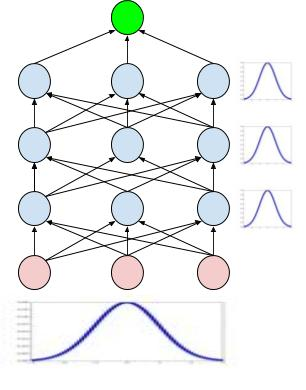
\includegraphics[scale=0.3]{images/BN_3.jpg}
					\end{figure}
					\begin{figure}
						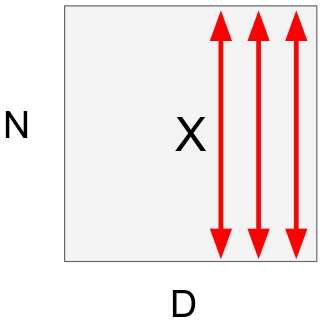
\includegraphics[scale=0.25]{images/batch.png}
					\end{figure}
				}
			}
		\end{overlayarea}
		
		\column{0.65\textwidth}
		\begin{overlayarea}{\textwidth}{\textheight}
			\begin{itemize}
				\justifying
				\only<1-8>{
					\only<1->{\item It would help if the pre-activations at each layer were unit gaussians}
					\only<5->{\item Why not explicitly ensure this by standardizing the pre-activation ?
						\begin{center}
							$\hat{s_{ik}} = \frac{s_{ik} - E[s_{ik}]}{\sqrt{var(s_{ik})}}$
						\end{center}}
					\only<6->{\item But how do we compute E[$s_{ik}$] and Var[$s_{ik}$]?}
					\only<7->{\item We compute it from a mini-batch}
					\only<8->{\item Thus we are explicitly ensuring that the distribution of the inputs at different layers does not change across batches}}
			\end{itemize}
		\end{overlayarea}
	\end{columns}
\end{frame}

%%%%%%%%%%%%%%%%%%%%%%%%%%%%%%%%%%%%%%%%%%%%%%%%%%%%%%%%%%%%%%%%%%%%%%%%%%%%%%%%%%%%%%%%%

\begin{frame}
	\begin{columns}
		\column{0.35\textwidth}
		\begin{overlayarea}{\textwidth}{\textheight}
			\only<2->{
				\begin{figure}
					\centering
					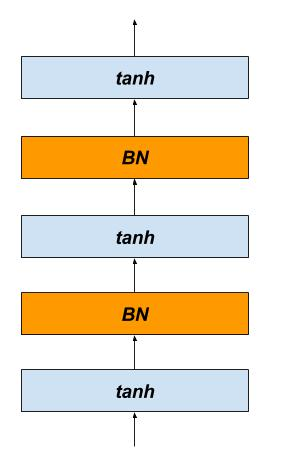
\includegraphics[scale=0.3]{images/BN.jpg}
					\label{fig:my_label}
				\end{figure}}
		\end{overlayarea}
		\column{0.65\textwidth}
		\begin{overlayarea}{\textwidth}{\textheight}
			\begin{itemize}
				\justifying
				\only<1-4>{
					\only<1-> {\item This is what the deep network will look like with Batch Normalization}
					\only<2->{\item Is this legal ?}
					\only<3->{\item Yes, it is because just as the $tanh$ layer is differentiable, the Batch Normalization layer is also differentiable}
					\only<4->{\item Hence we can backpropagate through this layer}
				}
			\end{itemize}
		\end{overlayarea}
	\end{columns}    
\end{frame}

\if 0
	\begin{frame}
		\begin{columns}
			\column{0.65\textwidth}
			\begin{overlayarea}{\textwidth}{\textheight}
				\begin{figure}
					\centering
					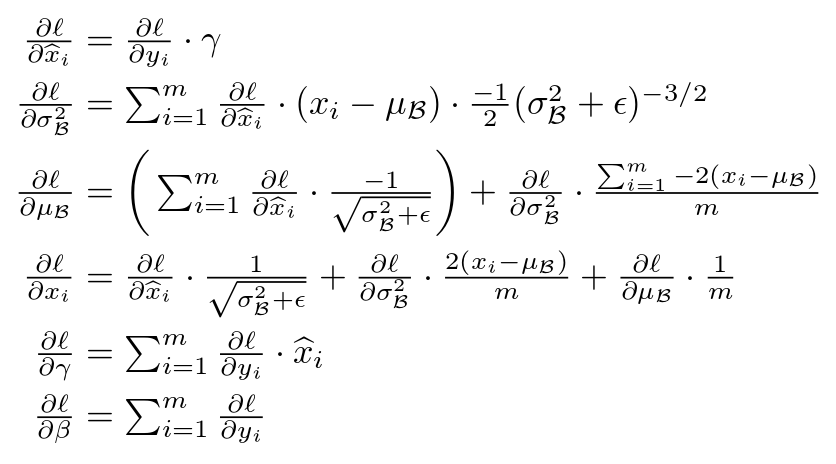
\includegraphics[scale=0.3]{images/equations.png}

					\caption{Differentiation Equations for Batch Normalization}
					\label{fig:my_label}
				\end{figure}
				
				%\begin{itemize}
					%\justifying
					%\only<1-6>{
					%\only<1->{\item $\frac{\partial \ell}{\partial \hat{x_i}} = 
					%\frac{\partial \ell}{\partial y_i}\gamma$
					%}
					%\only<2->{\item $\frac{\partial \ell}{\partial %\sigma_{B}^{2}} = \sum\limits_{i=1}^m \frac{\partial %\ell}{\partial \hat{x_i}}.(x_i - %u_B).\frac{-1}{2}{(\sigma_B^2 + \epsilon)}^{-3/2} $}}
					%\only<3->{\item $$}
				%\end{itemize}
			\end{overlayarea}
		\end{columns}
	\end{frame}
\fi 

\begin{frame}
	\begin{columns}
		
		\column{0.35\textwidth}
		\begin{overlayarea}{\textwidth}{\textheight}
			\onslide<1->{
				\begin{figure}
					\centering
					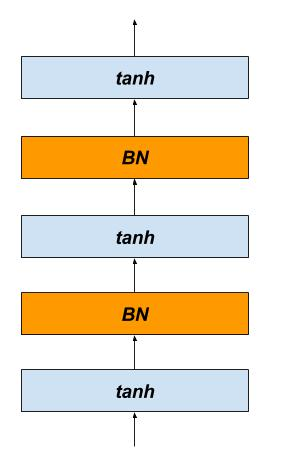
\includegraphics[scale=0.3]{images/BN.jpg}
					\label{fig:my_label}
				\end{figure}}
			\onslide<4->{
				$\gamma^{k}$ and $\beta^{k}$ are additional parameters of the network.
			}
		\end{overlayarea}
		\column{0.65\textwidth}
		\begin{overlayarea}{\textwidth}{\textheight}
			\begin{itemize}
				\justifying
				\onslide<1-6>{
					\onslide<1->{\item Catch: Do we necessarily want to force a unit gaussian input to the $tanh$ layer?}
					\onslide<2->{\item Why not let the network learn what is best for it?}
					\onslide<3->{\item After the Batch Normalization step add the following step:
						\begin{center}
							$y^{(k)} = {\gamma}^{k}\hat{s_{ik}} + \beta^{(k)}$
						\end{center}}
					
					\onslide<4->{\item What happens if the network learns:
						\begin{center}
							$\gamma^{k} = \sqrt{var(x^{k})}$
						\end{center}
						\begin{center}
							$\beta^{k} = E[x^{k}]$
						\end{center}
				}}
				\onslide<5->{\item We will recover $s_{ik}$}
				\onslide<6->{\item In other words by adjusting these additional parameters the network can learn to recover $s_{ik}$ if that is more favourable}
			\end{itemize}
		\end{overlayarea}
	\end{columns}
\end{frame}

%%%%%%%%%%%%%%%%%%%%%%%%%%%%%%%%%%%%%%%%%%%%%%%%%%%%%%%%%%%%%%%%%%%%%%%%%%%%%%%%%%%%%%%%%		

\begin{frame}
	
	We will now compare the performance with and without batch normalization on MNIST data using 2 layers....
\end{frame}



\begin{frame}
	%  \begin{columns}
	%  \column{0.5\textwidth}
	\begin{overlayarea}{\textwidth}{\textheight}
		
		\begin{figure}
			\foreach \n in {0,...,19} {%
				\pgfmathsetmacro\result{int(\n * 5)}
				\pgfmathsetmacro\t{int(\n + 1)}
				
				\includegraphics<\t>[scale=0.15]{images/DancingPlots/1_BN/\result_second.jpg}
				\includegraphics<\t>[scale=0.15]{images/DancingPlots/1_no_BN/\result_second.jpg}
				\includegraphics<\t>[scale=0.15]{images/DancingPlots/Error/\result.png}
			}
		\end{figure}  
	\end{overlayarea}
	%\end{columns}
\end{frame}

%%%%%%%%%%%%%%%%%%%%%%%%%%%%%%%%%%%%%%%%%%%%%%%%%%%%%%%%%%%%%%%%%%%%%%%%%%%%%%%%%%%%%%%%%			

\begin{frame}
	
	\begin{block}{2016-17: Still exciting times}
		\begin{itemize}
			\justifying
			\onslide<1->{\item \textbf{Eve}n better optimization methods}
			\onslide<2->{\item Data driven initialization methods}
			\onslide<3->{\item Beyond batch normalization}
		\end{itemize}
	\end{block}
	
\end{frame}